\chapter{Algorithm Recognition}
\label{chap:ch3}

\section{Introduction}
Algorithm recognition is a problem in which we want to get the similar algorithm with similar semantics. In the programming language to prove that two programs are same or not is a undecidable problem and that cannot be solved deterministically. The benefits of algorithm recognition could be better maintenance of the codes, tagging the similar programs, code suggestion. etc.   A tool can be derive form this solution and can ease the problem faced by the software developer in the daily routine. With the advent of machine learning based approximation strategies, several attempts have been made to fruitfully address this problem.

% Classifying programs based on the problem statement or detecting if two programs solve the same purpose is undecidable as there is no algorithm exist to emulate this on a Turing Machine. With that said, it cannot be solved on a modern computer. However, it is rather important -- classification of programs based on functionality helps in better maintainance of codes, helps in better code suggestion, etc. With the advent of machine learning based approximation strategies, several attempts have been made to fruitfully address this problem.

Applying deep learning to classify programs was first carried out by Peng et al.~\cite{Peng:2015}, and then used by various others~\cite{tbcnn-aaai16,ncc,Chen:2019} to demonstrate the goodness of their representation to classify programs. 
However, most of these approaches~\cite{Peng:2015,tbcnn-aaai16,Chen:2019} are trained to solve the specific task of classifying programs (whose representations cannot generalize across other tasks).

In this work, we have used the IR2Vec to get the program representations. We have applying this representation in supervised as well as unsupervised setting and discuss in upcoming sections about the work done respectively.

\section{Supervised Learning}
Supervised Learning is the field of machine learning in which the model is trained against known label or tags. The model for a given data point can't predict any thing not mentioned in the vocabulary. There are some fixit numbers of label for a machine learning task.
\vk{Add more here..}

% \subsection{Background}
In case of the image classification, there is a image dataset and each image is labeled. We run the training using the given images as the input and predict the image label. Given the true value and predicted value, we calculate the loss which is used to update gradient.
\vk{Related work}

% \subsection{Methodology}
On a similar note, we try to classify programs so as to recognize algorithms. Here, given a program, the objective is to classify it to one of the known classes that it would belong. fig~\ref{fig:supervised-background}

\begin{figure}[t]
    \centering
    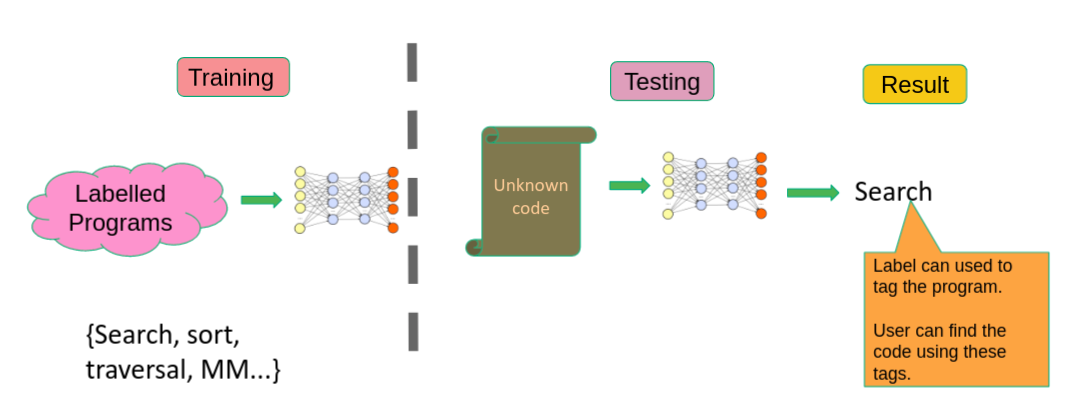
\includegraphics[scale=0.4]{figures/chapter-3/supervised_introduction.png}
    \caption{Algorithm Recognition in Supervised Way}
     \label{fig:supervised-background}
\end{figure}

% we want to predict to give algorithm class the program belong to.

We developed an classifier in TensorFlow\cite{tensorflow2015-whitepaper} which can classify the program respectively. 
\subsection{DataSet}
% We have selected the POJ-104 dataset\ref{tbcnn-aaai16} for our experiments. It has 104 type of different program which acts like class or label and each class has approximately ~500 programs. We have splitted this dataset into 3:1:1(training:testing:validation).

% ==================================================
We make use of the POJ-104 dataset introduced in Mou et al.~\cite{tbcnn-aaai16} for program classification. This dataset is obtained from Pedagogical Programming Open Judge (POJ/OJ) system, where the students submit the solutions to programming questions and the Open Judge system automatically evaluates those codes. 
Each programming question has an associated ID and many valid submissions across each ID. 
Each ID corresponding to a programming question forms a class, and all the submissions against the ID forms the data points of that class for classification problem. There are 104 such classes of C and C++ codes.

We follow the same data splitting strategy of earlier works by selecting 500 samples from each class randomly and splitting them in 3:1:1 ratio for training, testing and validation.
% ==================================================

% \subsection{Embedding Generation}

\subsection{Model}
% We used IR2Vec to generate the embedding for the input programs. For each program, we get a 300 dimension vector and its corresponding label. Such a vector is used as the input to the model.

% The first input layer expects a 300-dimension vector which is followed by simple three layered Multi-Level Precptron(MLP) with a softmax layer for output. The Categorical cross entropy Loss is used as the loss function and Adam as the optimizer. The whole training run for 100 epochs.

% ===================================================== (Can use directly)
For this classification task, we construct a simple three layered neural network which takes the vectors representing the programs of different classes as input and predicts the class as output. The neural network for this task consists of two stacked dense layers of 300 units each. Batch normalization~\cite{pmlr-v37-ioffe15-batchnorm} with ReLU as the activation function is used, with a dropout of 25\% as regularizer between each layer. The final layer is a softmax layer with the units equal to the number of classes of the programs. Adam optimizer with learning rate of 0.001 and categorical cross entropy is used as the loss function. Given an input vector, the network is trained to predict a class out of 104 classes of the input programs. 
% ===================================================

\subsection{Results}

We achieve an accuracy of 96.2\% with \textit{Flow-Aware} encodings. 
The results are compared with various methods that had used the same dataset for classifying the programs. We outperform the state-of-the-art methods on using a simpler neural network, whereas other methods use RNNs and LSTMs to achieve the results.
We obtain superior results by taking a very less training time of about \textit{one minute} per epoch when compared to the time taken by inst2vec of 1-2 hours per epoch on a P100 GPU, as claimed by the authors. 

As said earlier, the comparison is between TBCNN~\cite{tbcnn-aaai16}, inst2vec~\cite{ncc} and IR2Vec-Symbolic and IR2Vec-Flow-Aware.

% \begin{center}
\begin{table}[h]
\centering
  \caption{POJ-104 classification results}
%   \vspace*{-\baselineskip}
  \label{tab:pc_accuracy}   % \small
    \begin{tabular}{ccccc}
    \toprule
     & \textbf{TBCNN} & \textbf{inst2vec} & \textbf{IR2Vec-Flow-Aware}\\
        \hline
        \textbf{Accuracy} & 94\% & \textit{94.83\%\protect\footnotemark}  & \textbf{96.2\%} \\
    \bottomrule
    \end{tabular}
% \vspace*{-\baselineskip}
\end{table}
% \end{center}
 \footnotetext{This value is quoted by the authors in their paper.}


% \subsection{Visual Technique}
As mentioned above have 300 dimension vector and it reduce it's dimension to 2 dimensions using t-SNE\cite{}. Points which are similar to each other meant to be near to each other. The effectiveness of the encoding different instance to time during training is shown.

\begin{figure}[h]
    % \centering
\begin{subfigure}[b]{0.3\textwidth}
%   \centering
  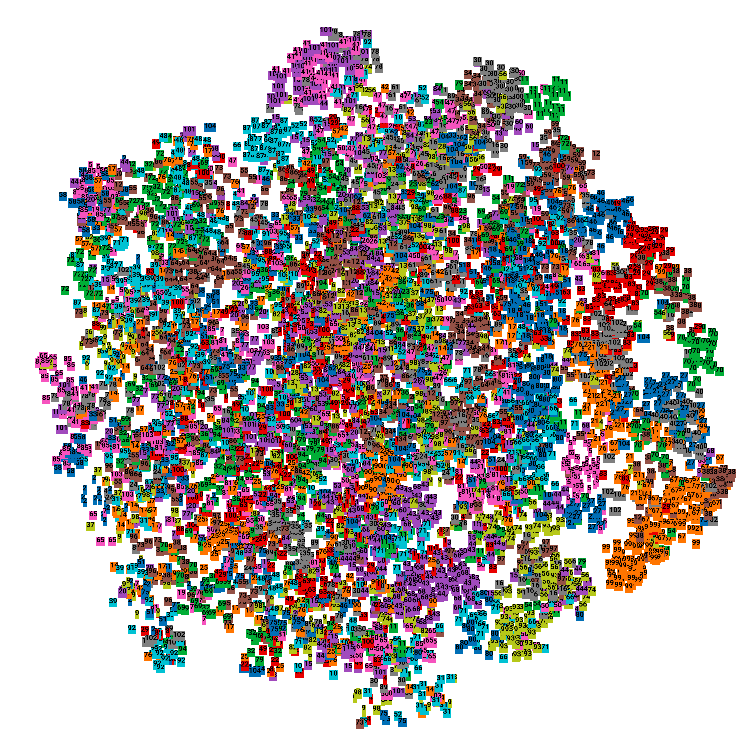
\includegraphics[width=\textwidth]{figures/untrained.png}  
  \caption{Untrained}
  \label{fig:0e}
\end{subfigure}
\hfill
\begin{subfigure}[b]{0.3\textwidth}
%   \centering
  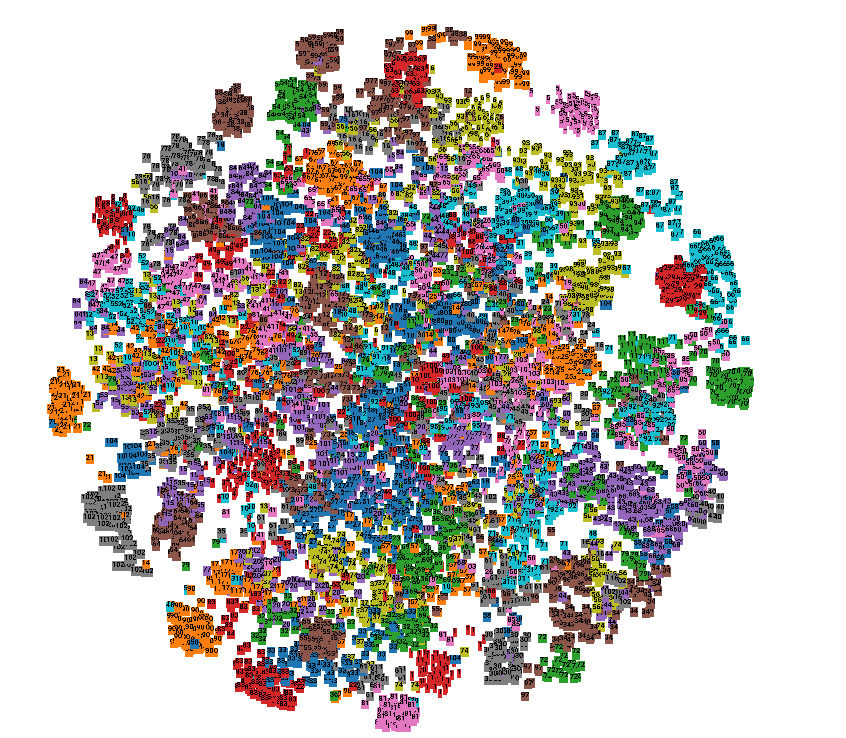
\includegraphics[width=\textwidth]{figures/5e_tsne.png}  
  \caption{After 5 Epochs}
  \label{fig:5e}
\end{subfigure}
\hfill
\begin{subfigure}[b]{0.3\textwidth}
%   \centering
  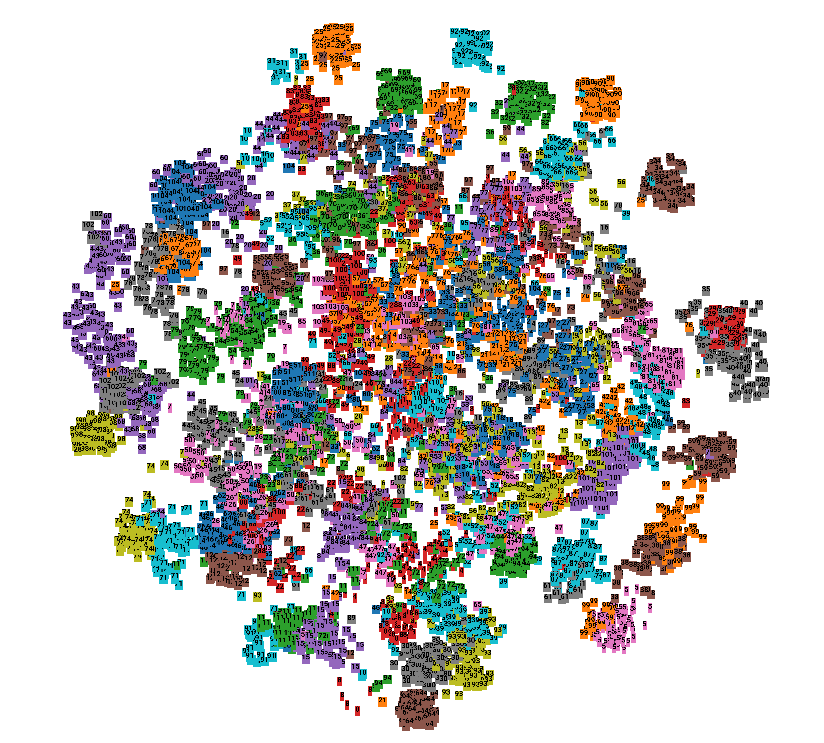
\includegraphics[width=\textwidth]{figures/full_tsne.png}  
  \caption{After 100 Epochs}
  \label{fig:100e}
\end{subfigure}
    \caption{Comparison of cluster at different instant}
    \vspace*{-\baselineskip}
    \label{fig:clusters}
\end{figure}

\begin{itemize}
    \item In Fig.~\ref{fig:0e}, we show the untrained data. It can be seen that points of similar labels are grouped together to some extent, though the clusters are not formed distinctly.
    % \vspace*{-0.4cm}

% It is a well accepted fact that the weights of the penultimate layer of the neural network represe the representation of 
% After training the classification model with the training data points for 5 epochs, we obtain the 

    \item In Fig.~\ref{fig:5e}, we show the plot formed by the learned output vectors that were taken from the last layer of the classification model after 5 epochs of the training for the same test data points. As it can be seen, on a minimalistic training, they quickly form better clusters.
    %   \vspace*{-0.4cm}
    \item At the end of training, after 100 epochs, the points form more distinct clusters as shown in Fig.~\ref{fig:100e}.
\end{itemize}

% Unsupervised Learning started
\section{Unsupervised Learning}


\subsection{Background}
Unsupervised learning is the machine learning technique that is used to train the model without labels. The clustering algorithm like KNN, K-means, hierarchical clustering, and others. 
	Learning used to happen based upon minimizing the intra-cluster distance and maximizing the inter-cluster distances. Similar data points stay near a similar point and far from the non-similar ones. This can be used for the inference of the unseen classes.
	
	As the Fig~\ref{fig:unsupervised-background}, given the set of unlabelled program and pass them through a  machine learning model. The model will try to form clusters of similar programs during the training. After training is done, we perform inference on the model, it try to assign the program to the best-suited cluster. This is a schematic diagram of the flow for better understanding.

	Few shot learning is a way of unsupervised learning in which while inference there is some data point in which the trained model adjusts the final prediction.

\begin{figure}[t]
    \centering
    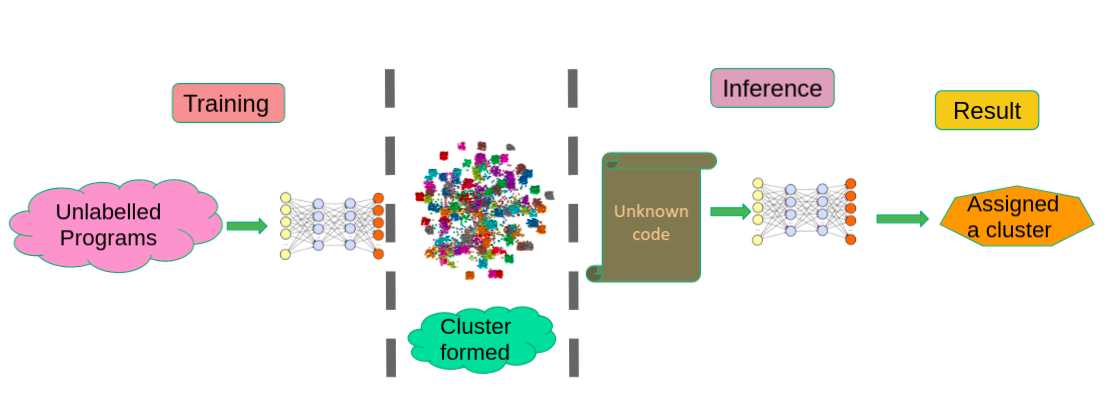
\includegraphics[scale=0.4]{figures/chapter-3/unsupervised.png}
    \caption{Algorithm Recognition in Unsupervised Way}
     \label{fig:unsupervised-background}
\end{figure}

\subsection{Few-Shot Learning}
	    It is a type of unsupervised learning, in which the training phase has two sets i.e support set and a Query set. The training happens in task. Each task consist of N classes and K datapoint in the support set and N classes in the support set. Each task has a mutually exclusive set i.e. all the N classes are not part of another task.(fig~\ref{fig:unsupervised-fewshot})
% 	Training

    A task is given to the model and support set is passed to the model. Now to see how much the model learns after first task, we run it on the query set for which we knew the label. The datapoint belonging to same class should lie near to each other. In the example fig[], Cat in the query set of task 1 should lie near the cat cluster of the support set and respectively for other classes.
	
	The Loss function is formulated in terms of the distance metric. If the query set is far apart during training then more is the loss and that needs to backpropagate for the better learning of the next task or batch.

\begin{figure}[t]
    \centering
    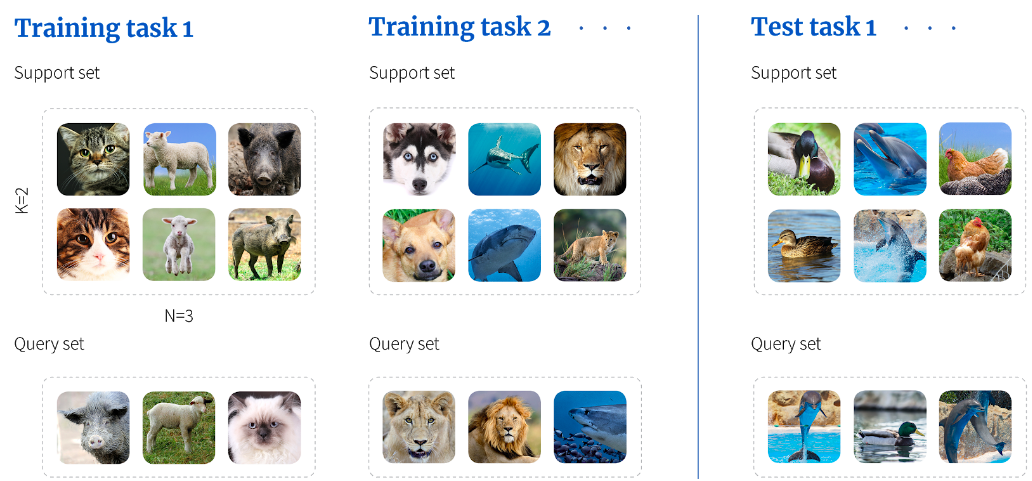
\includegraphics[scale=0.4]{figures/chapter-3/unsupervised_few_shot.png}
    \caption{Few shot Learning Example}
     \label{fig:unsupervised-fewshot}
\end{figure}


\begin{figure}[t]
    \centering
    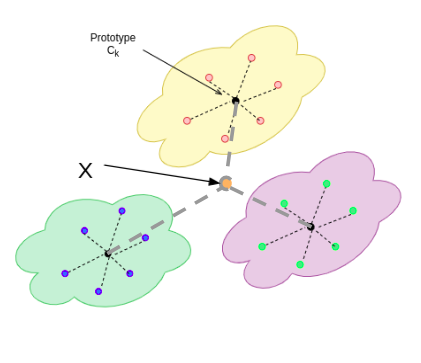
\includegraphics[scale=0.5]{figures/chapter-3/prototypes.png}
    \caption{Prototypes}
     \label{fig:unsupervised-prototypes}
\end{figure}

\subsection{Prototypical Networks}
Prototypical Networks is a way for few-shot classification where it try to generalize the model to the unseen label at the time of training. They have proposed a loss function known as Prototypical Loss Sec~\ref{sec:algo:proto:loss} and use it train the network. They map the input embedding a new latent space where similar points are nearer. $S_{k}$ is the support set for class \textit{k}, $f_{\phi}$ is the neural network which map input to the latent space.

\subsubsection{Prototype}
During the training phase when the support set is passed the model. Each class forms an aggregate point from other participating points and known as the prototype (Fig.~\ref{fig:unsupervised-prototypes}). In equation~\ref{eq:1}, prototype($c_{k}$) is been calculated for each class respectively. \vk{More here}

 
\begin{equation} \label{eq:1}
c_{k} = \frac{1}{|S_{k}|}  \sum_{(x_{i},y_{i}) \epsilon S_{k}}  f_{ \phi }(x_{i})
\end{equation}

\subsubsection{Loss Function}\label{sec:algo:proto:loss}
During the training phase, datapoint from form each class of the Query set to evaluated against the respective prototype. The loss function forms the probability distribution of a prototype($c_{k}$) given a point \textbf{x} . Using the square euclidean metric to calculate the distance between them. Less is the distance, higher  is the probability of the point x that it belongs to the respective prototype. Loss function is negative log-probability of $p_{\phi}$ from Eq.~\ref{eq:2}\vk{Equation}

\begin{equation}\label{eq:2}
p_{ \phi }(y = k | x) =  \frac{exp(-d(f_{\phi}(x), c_{k}))}{\sum_{k^{'} }exp(-d(f_{\phi}(x), c_{k^{'}}))} 
\end{equation}

\subsection{Program categorization for unseen programs}
Inspring from the work mentioned above, we want to apply the same technique to the programs. We make the required changes to the Prototypical Networks~\cite{protonet:NIPS2017} to work for the programs presentations.  

\subsection{Dataset}
We have selected the POJ-104 dataset\cite{tbcnn-aaai16} for our experiments. It has 104 type of different program which acts like class or label and each class has approximately ~500 programs. We have split this dataset into Train: Test: Val →  1-80 classes (80): 81-94 classes (14): 95-104 classes (10).

\subsection{Model Architecture}
The implementation was done using PyTorch in python. The first input layer expects a 300-dimension vector which is followed by a simple three-layered Multi-Level Perceptron(MLP) with a softmax layer for output. The Prototypical Loss Function~\ref{sec:algo:proto:loss} is used as the loss function and Adam optimizer. The whole training runs for 100 epochs.

\subsection{Results}
We have calculate the accuracy for four configuration. The \textit{\textbf{N way}} is the number of the classes used in each task and \textit{\textbf{K shot}} is the number datapoint  of each class are being used. See the Tab.~\ref{tab:unsupervised-acc}.
\begin{table}[h]
\begin{tabular}{lllll}
\hline
\multirow{2}{*}{\textbf{POJ Experiment}} & \multicolumn{2}{l}{\textbf{5 ways}} & \multicolumn{2}{l}{\textbf{10 ways}} \\
 & \textbf{1 Shot} & \textbf{5 Shot} & \textbf{1 Shot} & \textbf{5 Shot} \\
\hline
Test Accuracy \% & 78.47 & 89.66 & 80.9 & 91.27 \\
\hline
\end{tabular}
\centering
\caption{Compare the accuracy percentage.}
\label{tab:unsupervised-acc}
\end{table}

\vk{Conclusion}